\chapter{Model Evaluation and Results Analysis}
\label{chap:Chapter4}

This chapter provides an in depth analysis of the performance and results obtained from testing the models in two distinct environments: the local testing environment and the live testing environment.

\section{Local Testing Environment}

In the local testing environment, the models were evaluated using a dataset that was split into training and testing subsets

Due to hardware limitations\footnote{Training a single alert takes 10 to 15 minutes, making it impractical to train on 100k alerts in a reasonable timeframe.}, the RL model was not tested on this environment, therefore, the results presented in this section are only of the RF model's performance and its evolution from Version 1 to Version 11.

The RF model was trained and tested on the dataset, and its performance was measured using metrics such as accuracy, precision, recall, and F1-score.
\begin{itemize}
    \item \textbf{Accuracy:} The proportion of correctly classified alerts out of the total alerts.
    \item \textbf{Precision:} The ratio of true positive predictions to the total predicted positives, indicating the model's ability to avoid false positives.
    \item \textbf{Recall:} The ratio of true positive predictions to the total actual positives, reflecting the model's ability to capture all relevant alerts.
    \item \textbf{F1-score:} The harmonic mean of precision and recall, providing a balanced measure of the model's performance.
\end{itemize}

The values for all the metrics are based on the final results from training. 
Since, after training the model, that same model is tested against a test data subset, it is possible to get values for the model's performance and accuracy.

Table~\ref{tab:results_comparative} shows the values for the metrics of Version 1 and Version 11, showing the evolution of the model from the first to the last version.

\clearpage

\begin{table}[h!]
    \centering  
    \caption{Model Performance Metrics Comparison: Version 1 vs. Version 11}
    \label{tab:results_comparative}
    \begin{tabular}{@{}ccccc@{}}
        \toprule
        \multirow{2}{0em}{} & \multicolumn{2}{c}{\textbf{Priority}} & \multicolumn{2}{c}{\textbf{Taxonomy}} \\
        & \textbf{Version 1} & \textbf{Version 11} & \textbf{Version 1} & \textbf{Version 11} \\
        \hline
        \textbf{Accuracy} & 82\% & 90\% & 82\% & 90\% \\
        \textbf{Precision} & 82\% & 89\% & 81\% & 90\% \\
        \textbf{Recall} & 80\% & 89\% & 65\% & 90\% \\
        \textbf{F1-Score} & 82\% & 89\% & 69\% & 90\% \\
        \bottomrule
    \end{tabular}
\end{table}

From the table, it is evident that Version 11 demonstrates notable improvements over Version 1 in all metrics. Specifically:

\begin{itemize}
    \item \textbf{Accuracy:} Both priority and taxonomy classifications improved from 82\% in Version 1 to 90\% in Version 11, indicating a higher proportion of correctly classified alerts overall.
    \item \textbf{Precision:} The precision for priority classification increased from 82\% to 89\%, and for taxonomy classification, it rose from 81\% to 90\%. Making it clear that Version 11 is better at minimizing false positives.
    \item \textbf{Recall:} A significant improvement is observed in recall, particularly for priority classification, which increased from 65\% in Version 1 to 90\% in Version 11. This indicates that the model is now more effective at identifying true positives, especially for minority or low frequency categories.
    \item \textbf{F1-Score:} The F1-Score, which balances precision and recall, also improved from 69\% to 90\% for priority classification, reflecting the overall enhancement in the model's robustness.
\end{itemize}

These improvements highlight the evolution of the model's ability to handle complex classification tasks, particularly in addressing challenges associated with low frequency categories. 
The enhanced recall for minority classes is particularly noteworthy, as it demonstrates the model's capacity to reduce bias and improve fairness in predictions.

Besides accuracy, recall is a fundamental factor, as being able to correctly identify an alert for what it truly is—whether in terms of priority or taxonomy—is critical. 
Confusing a P1 (high priority) with a P3 (low priority) can have serious consequences, potentially leading to delayed responses or misallocated resources.

The confusion matrix is a fundamental tool in evaluating the performance of classification models, providing a detailed breakdown of the model's predictions across all categories. 
It is a tabular representation that contrasts the actual labels with the predicted labels, allowing for the identification of true positives, false positives, true negatives, and false negatives for each class. 

This granular insight is crucial for understanding the model's strengths and weaknesses, particularly in distinguishing between similar or imbalanced classes. 
The confusion matrices presented in this section are derived from the same output\footnote{All outputs relevant to this section can be found in Appendix~\ref{AppendixA}.} as the previously discussed performance metrics, generated during the execution of the command that initiates the training of the RF model.

Therefor, analyzing the confusion matrices is essential to understand the model's performance in detail.
The confusion matrices provide a visual representation of the model's performance, allowing us to see how well the model classifies each category and where it tends to make mistakes.

Figures~\ref{fig:confusion_priority_v1} and \ref{fig:confusion_priority_v11} illustrate the evolution of the model's performance in priority classification from Version 1 to Version 11. 

\begin{figure}[h!]
    \centering
    \begin{minipage}{0.49\textwidth}
        \centering
        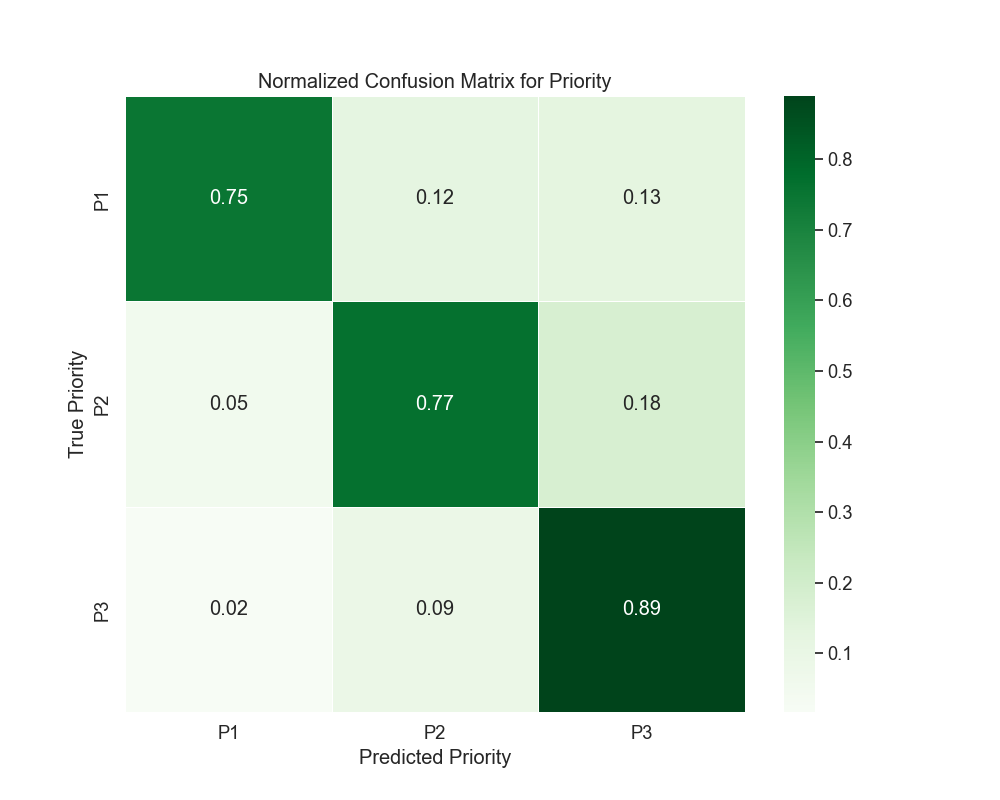
\includegraphics[width=\textwidth]{ch4/assets/v1_confusion_priority.png}
        \caption{Confusion Matrix for Priority (Version 1)}
        \label{fig:confusion_priority_v1}
    \end{minipage}
    \hfill
    \begin{minipage}{0.49\textwidth}
        \centering
        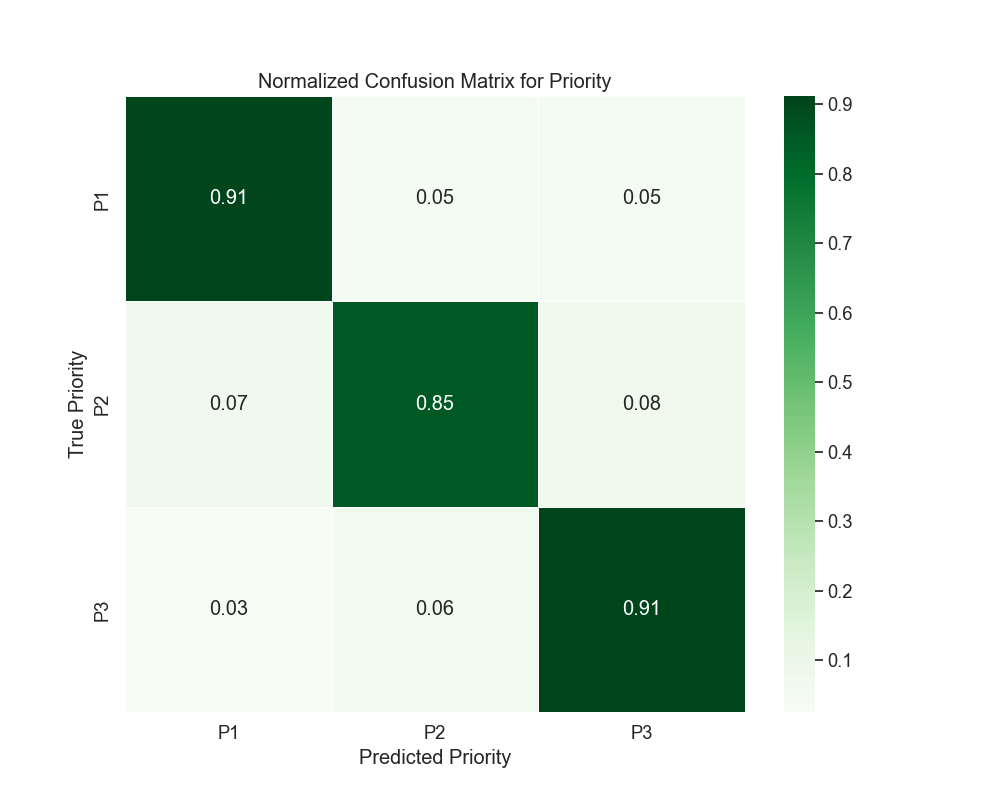
\includegraphics[width=\textwidth]{ch4/assets/v11_confusion_priority.png}
        \caption{Confusion Matrix for Priority (Version 11)}
        \label{fig:confusion_priority_v11}
    \end{minipage}
\end{figure}

In Version 1, the confusion matrix (Figure~\ref{fig:confusion_priority_v1}) reveals notable misclassifications, particularly between P1 and P2 categories. 
The recall values for P1 and P2 were 0.75 and 0.77, respectively, while P3 achieved a higher recall of 0.89, indicating relatively better performance for lower priority classes. 

In contrast, Version 11 (Figure~\ref{fig:confusion_priority_v11}) demonstrates significant improvements, achieving recalls of 0.91 for P1, 0.85 for P2, and 0.91 for P3. 
These enhancements reflect a substantial reduction in misclassifications, particularly between P1 and P2, showcasing the model's improved ability to differentiate between priority levels. 

The key advancements from Version 1 to Version 11 are evident in the increased recall for P2, which rose from 0.77 to 0.85, and for P3, which improved from 0.89 to 0.91. 
These results underscore the model's enhanced accuracy and robustness in handling priority based predictions, particularly for categories that were previously challenging to classify accurately.

The same analysis can be applied to taxonomy classification, where the confusion matrices provide insights into the model's performance across different categories.

In Version 1 (Figure~\ref{fig:confusion_taxonomy_v1}), the model's performance was somewhat lacking, especially with low frequency categories. 
For example:

\begin{itemize}
    \item \textbf{"Abusive Content"} had a recall of only \textbf{0.19}, meaning that a substantial portion of this class was misclassified.
    \item \textbf{"Fraud"} performed well with \textbf{0.95} recall, demonstrating that the model successfully identifies most instances of fraud.
    \item \textbf{"Vulnerable"} had \textbf{0.36} recall, indicating the model struggled to identify alerts related to vulnerabilities.
    \item \textbf{"Intrusions"} also performed poorly with \textbf{0.54} recall.
    \item \textbf{"Information Gathering"} was significantly more challenging with \textbf{0.47} recall, suggesting that the model could not detect a substantial portion of critical security threats in this category.
\end{itemize}

\begin{figure}[h!]
    \centering
    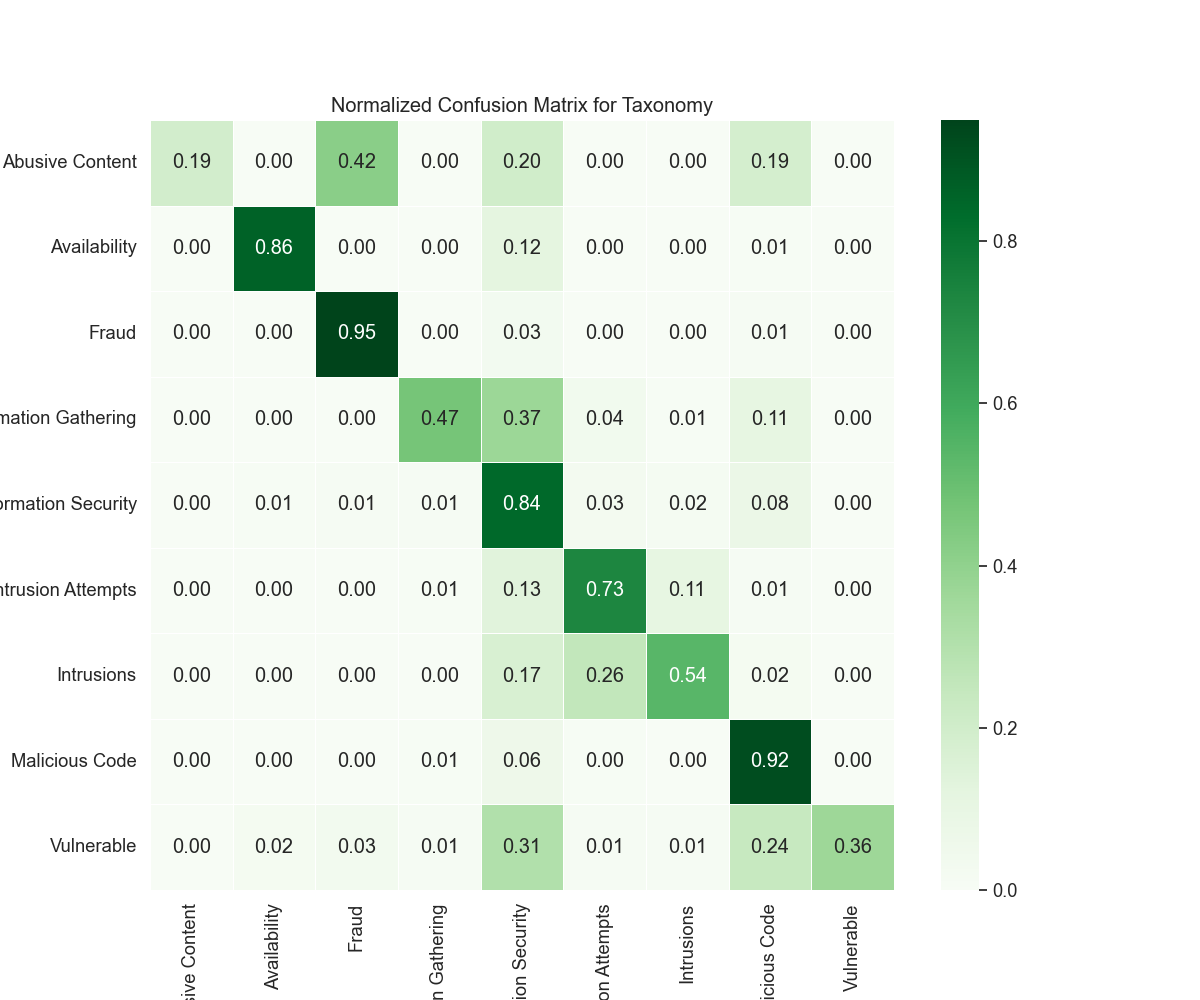
\includegraphics[width=0.8\textwidth]{ch4/assets/v1_confusion_taxonomy.png}
    \caption{Confusion Matrix for Taxonomy (Version 1)}
    \label{fig:confusion_taxonomy_v1}
\end{figure}

Whereas, in Version 11 (Figure~\ref{fig:confusion_taxonomy_v11}), the model's performance improved significantly across all categories.

In Version 11, several key improvements were made:

\begin{itemize}
    \item \textbf{"Abusive Content"} showed a dramatic improvement in recall to \textbf{0.46}, almost a threefold increase. The model is now better at identifying such content, which is crucial in detecting harmful communications or activity.
    \item \textbf{"Fraud"} maintained a high recall of \textbf{0.94}, demonstrating that the model continues to perform well in this critical category.
    \item \textbf{"Vulnerable"} showed a notable improvement in recall to \textbf{0.99}, addressing the initial weakness seen in Version 1. This is essential for detecting vulnerabilities and minimizing risks.
    \item \textbf{"Intrusions"} also improved significantly to \textbf{0.89}, indicating that the model is now better at identifying intrusion attempts, which are often targeted threats.
    \item \textbf{"Information Gathering"} improved from \textbf{0.47} in Version 1 to \textbf{0.94} in Version 11, reflecting a better capability to identify security related alerts, which was a major challenge in the previous version.
\end{itemize}

\begin{figure}[h!]
    \centering
    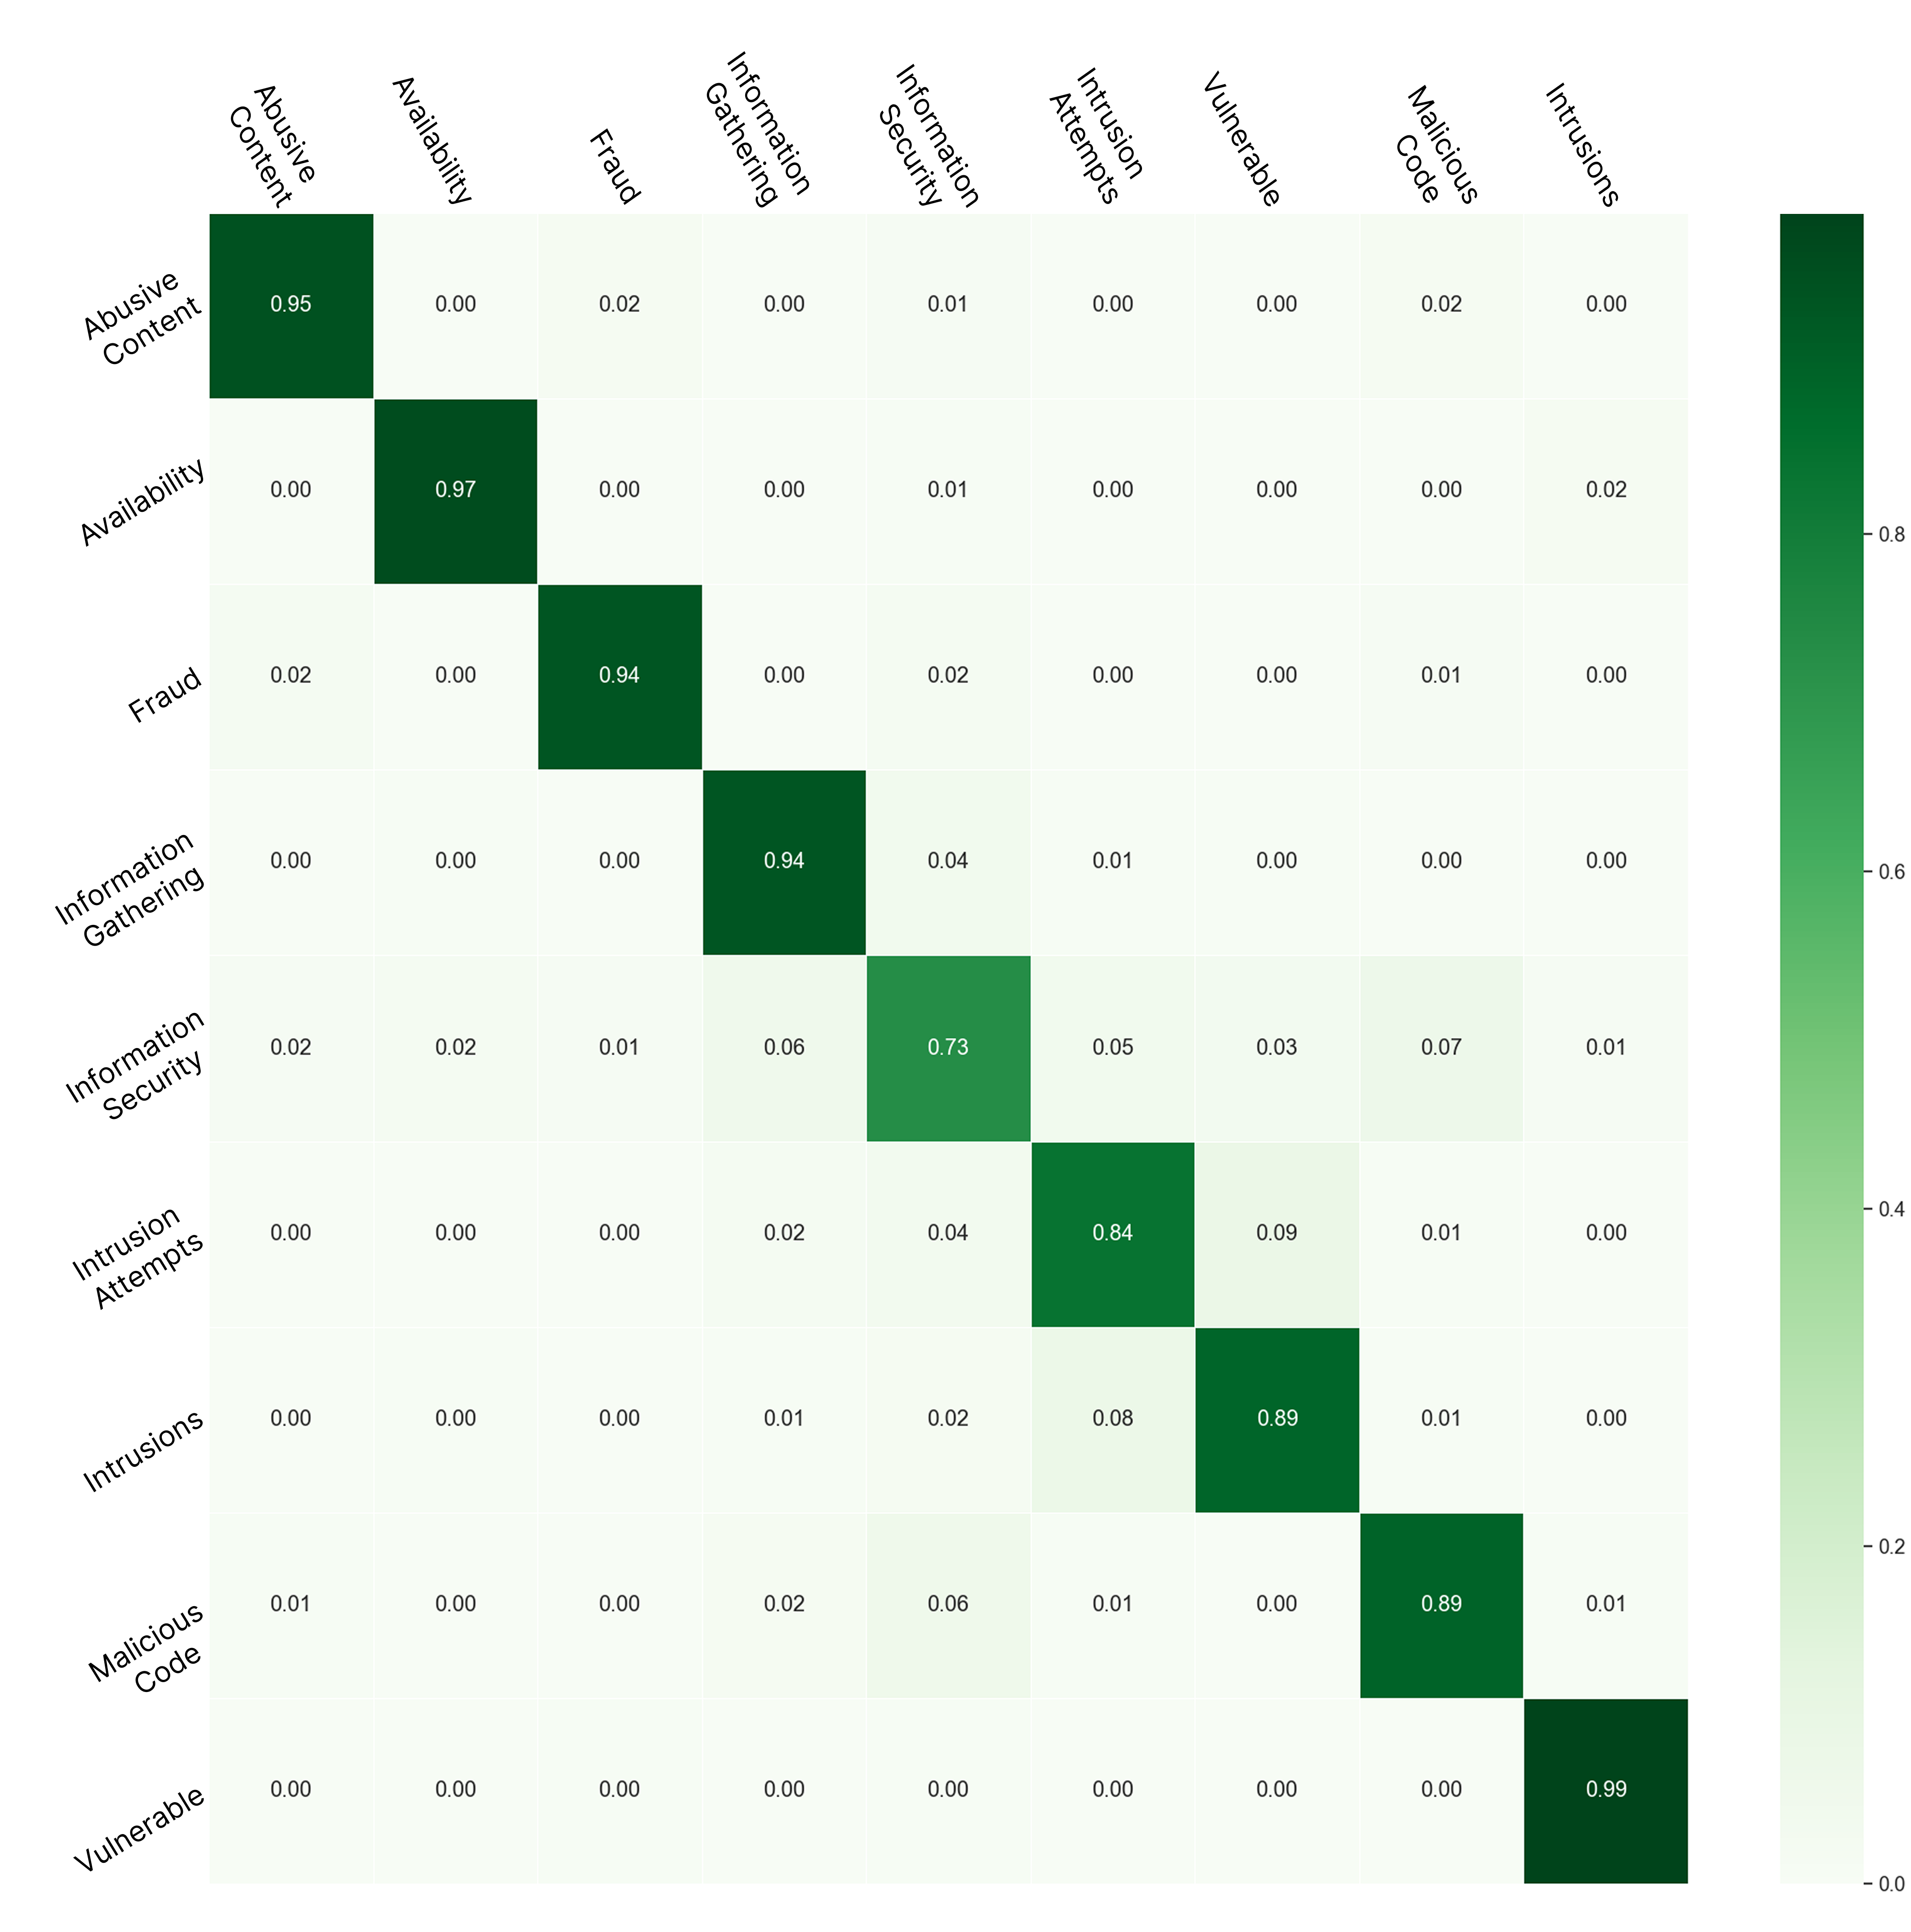
\includegraphics[width=\textwidth]{ch4/assets/v11_confusion_taxonomy.png}
    \caption{Confusion Matrix for Taxonomy (Version 11)}
    \label{fig:confusion_taxonomy_v11}
\end{figure}

The improvements in recall across all categories in Version 11 indicate that the model is now more effective at identifying relevant alerts, particularly in low frequency categories.
This is crucial for ensuring that the model can accurately classify and prioritize alerts, especially in cases where certain categories may have been previously overlooked or misclassified.

\section{Live Testing Environment}

The live testing environment aims to simulate real world deployment, where the models are evaluated based on their actual performance in the company's infrastructure. 
In this environment, both the RF and RL models are expected to be used. 
However, unlike the local environment where testing was done solely on the RF model, the live environment will also involve continuous training of the RL model. 
As feedback is gathered, the RL model is expected to improve its performance over time.

For the live testing, the application will not be evaluated separately on the RF and RL models but will instead use both models as part of an integrated system. 
During this phase, feedback from real time predictions will be used to adjust and fine tune the RL model's decisions. 
The expectation is that with time, the RL model will show improvements in its ability to predict priority and taxonomy, surpassing the performance of the initial RF model version.

This section describes the deployment and validation of the proposed system in a real world setting, within the infrastructure of ArtResilia. 
The goal was to evaluate the performance and operational viability of the integrated solution under realistic conditions. 
This included the full deployment of the API, containerized services, integration with IBM QRadar SOAR via playbooks, and the subsequent observation and resolution of runtime constraints.

\subsection{Deployment Architecture and Integration Workflow}

Following the successful training of the RF model and implementation of the full API according to previously agreed specifications, a Swagger documentation interface was developed to facilitate integration with the security orchestration team. 
This interface described the available endpoints and their expected input/output structure.

The integration and deployment process involved several key steps:

\begin{itemize}
    \item \textbf{Swagger Delivery:} The Swagger API documentation was sent to the responsible party at ArtResilia. This enabled the creation of a custom playbook within IBM QRadar SOAR to handle ticket classification and feedback submission.
    \item \textbf{VM Provisioning:} In parallel, a new virtual machine (VM) was prepared to host the deployed solution. Unlike the local development environment with 16GB of RAM, the testing VM had only 4GB of RAM. This difference significantly impacted the resource management strategy, particularly during RL model training.
    \item \textbf{Dockerized Deployment:} To ensure portability and simplify environment replication, Docker was used to containerize the application. This approach offers several advantages over native installation, including consistent runtime environments, isolation of dependencies, simplified updates, and ease of monitoring and scaling individual services. The deployed architecture consisted of four containers:
    \begin{enumerate}
        \item \textbf{API and Bot Container:} Handles real time prediction requests and exposes the REST endpoints.
        \item \textbf{Celery Worker Container:} Executes background tasks such as RL model training based on analyst feedback.
        \item \textbf{Flower Monitoring Container:} Provides a web interface for monitoring Celery tasks and Redis queue status.
        \item \textbf{Redis Container:} Serves as the message broker between the API and Celery worker.
    \end{enumerate}
    \item \textbf{Shared Volume and Model Caching:} A shared Docker volume was mounted between the API and Celery containers to allow direct access to cached model files. This ensured consistency when loading and updating model versions during feedback based training.
    \item \textbf{Embedding Model Caching:} Due to strict firewall configurations enforced via iptables, the VM had no internet access outside the ArtResilia VPN. Therefore, pre-trained models such as Sentence-BERT were bundled directly into the Docker image to prevent the need for online downloads during runtime.
    \item \textbf{Access Control via NGINX:} An NGINX reverse proxy was configured to provide external access to the API and the Flower dashboard. Basic HTTP authentication was enforced to restrict access to authorized users only.
\end{itemize}

\subsection{SOAR Integration via Playbook}

The integration with IBM QRadar SOAR was implemented through an asynchronous playbook, designed to avoid disruption of SOC workflows in case the system became unavailable. The playbook behavior can be summarized as follows:

\begin{itemize}
    \item When a new ticket is created, a GET request is sent to the API to retrieve the predicted taxonomy and priority.
    \item These predictions are displayed in the SOAR web interface in dedicated fields labeled ``Predicted Taxonomy'' and ``Predicted Priority''.
    \item Upon ticket closure, the actual analyst defined values for taxonomy and priority are submitted to the API via a POST request to trigger the feedback learning mechanism.
    \item The playbook was configured to execute asynchronously. This ensures that even if the prediction system is temporarily offline, the SOAR platform continues to operate normally, skipping the classification step without interruption.
\end{itemize}

\subsection{Runtime Challenges and Solutions}
Upon initial deployment, the system began to operate successfully, processing classification requests for incoming tickets.
However, problems emerged when the RL model attempted to train based on the feedback data. 

\paragraph{Memory Problem}
The Celery container crashed due to memory exhaustion, consuming over 4GB of RAM plus all available swap space.

To address this problem:
\begin{itemize}
    \item A new VM with 8 GB of RAM was provisioned, but the same crashes reoccurred during RL training.
    \item Since further increasing the VM's memory was not a sustainable solution, a custom memory management strategy was developed using Python's built in gc (garbage collector) module.
\end{itemize} 

\paragraph{Solution - Custom Garbage Collection Strategy}

To reduce memory usage, a targeted cleanup process was applied at the end of each Celery training task. 
This was done by explicitly deleting large intermediate variables and invoking Python's garbage collector.

\vspace{0.2cm}
\noindent
\begin{minipage}{\linewidth}
\begin{minted}{python}
del {variable_name}
gc.collect()
\end{minted}
\captionof{listing}{Custom Garbage Collection Strategy}
\label{lst:custom_gc_strategy}
\end{minipage}
\vspace{0.1cm}

The code in Listing~\ref{lst:custom_gc_strategy} performs explicit memory management in Python. 
Line 1 explicitly deletes a variable from memory, removing its reference and making it eligible for garbage collection. 
Line 2 then manually triggers Python's garbage collector to immediately reclaim memory from objects that are no longer referenced.

This strategy ensured that each training session released its memory footprint before the next one started. 
After implementing this fix, memory usage was stabilized and kept under 6GB, preventing further crashes and allowing uninterrupted operation.

\subsection{Results and Observations}

With the system stabilized, the final step was to let it run uninterrupted for a continuous period to gather performance metrics. 
During this period, the system operated in parallel with the standard SOC workflow, producing live predictions and processing analyst feedback asynchronously.

\subsubsection{Accuracy and Learning Curves Over Time}

Over the course of 15 days of uninterrupted live testing, a total of 519 alerts were processed. 
The model made predictions for each alert, and all of these predictions received analyst feedback. 
Based on this feedback, training tasks were dispatched to the RL model, enabling incremental learning.

In this evaluation, a prediction was considered "correct" only when both the priority and taxonomy classifications matched the analyst submitted values.
The following figures used the data explained in appendix~\ref{AppendixB} to visualize the model's performance over time.

\begin{figure}[h!]
    \centering
    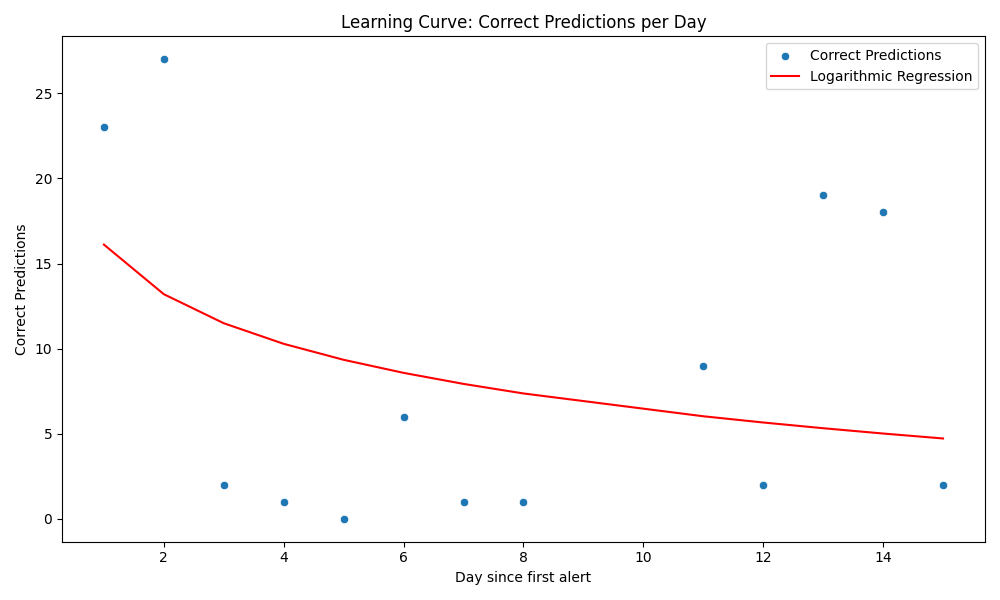
\includegraphics[width=0.85\textwidth]{ch4/assets/learning_curve_corrects.png}
    \caption{Correct Predictions per Day (Priority + Taxonomy)}
    \label{fig:learning_curve_corrects}
\end{figure}

Figure~\ref{fig:learning_curve_corrects} shows the number of correct predictions made each day. 
While the model had strong performances on Day 0, Day 1, and Day 10, it also exhibited weaker results on Days 2 through 7. 
A logarithmic regression line was fitted to capture the general trend across the observation window.
Rather than the expected upward curve that would suggest a growing influence of the RL model refining the baseline RF predictions, the trend displays a slight decline.

This result differs with the intended behavior of the system, where RL was expected to gradually assume control from the RF model, leveraging historical feedback to increase accuracy and confidence.
Instead, the data suggests that within the limited 15 day window, the RL component had not yet reached sufficient knowledge to impact performance.
Still, this graph offers valuable insight into how the hybrid RF+RL model performed in early deployment, and establishes a baseline for what an improving curve might look.

\begin{figure}[h!]
    \centering
    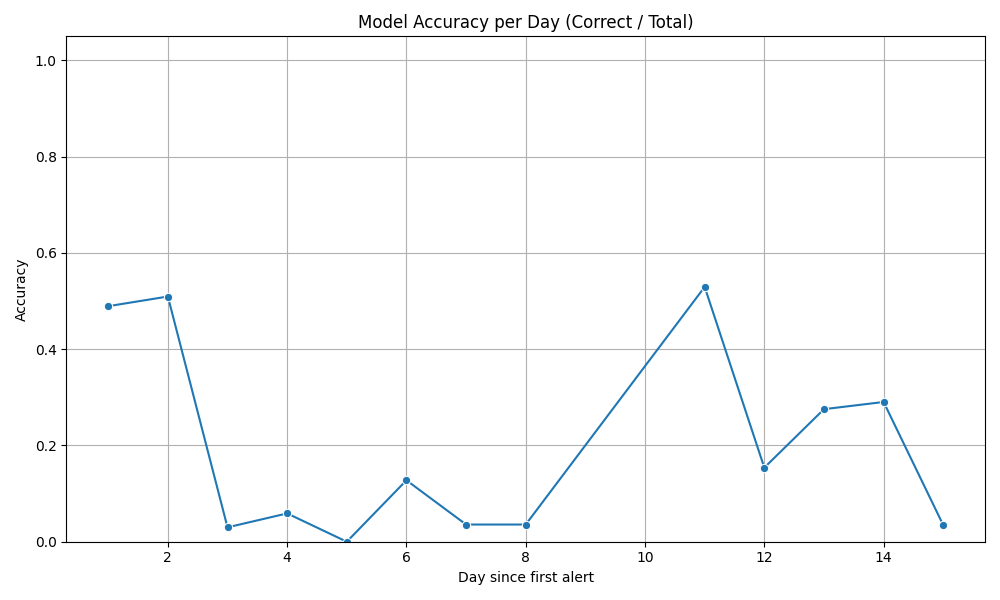
\includegraphics[width=0.85\textwidth]{ch4/assets/learning_curve_accuracy.png}
    \caption{Accuracy per Day (Both Labels Must Match)}
    \label{fig:learning_curve_accuracy}
\end{figure}

Figure~\ref{fig:learning_curve_accuracy} presents the model's daily accuracy, defined as the proportion of alerts for which both the predicted priority and taxonomy matched the analyst-submitted values. 
While this graph shows similar information to Figure~\ref{fig:learning_curve_corrects}, it provides a complementary perspective.

Whereas the previous figure illustrated the absolute number of correct predictions, this one accounts for the daily volume of processed alerts. 
For example, a day with only ten alerts might have a higher accuracy despite few total correct predictions, while a high volume day with modest accuracy may still result in many useful classifications. 
Together, these graphs offer a more complete picture of the system's behavior.

By observing both, one can distinguish between days where the system performed well due to higher precision versus days where volume may have tilted the perception of success. 
Notably, the decline seen in the accuracy curve aligns with the drop in absolute correct predictions, reinforcing the notion that performance was inconsistent during the early testing phase.

This pattern diverges from the ideal learning curve expected in RL environments. 
Ideally, as the RL model accumulates feedback, its corrections should incrementally improve classification outcomes producing an upward trend in both accuracy and correct predictions over time. 

The likely cause is the relatively short evaluation window. 
In just 15 days of operation, the RL model lacked sufficient data to learn with confidence from past feedback. 
As a result, predictions remained largely influenced by the static RF model, which was trained offline and does not adapt over time.

Despite this, both images, not only document the initial performance of the RF+RL hybrid system, but also provide a benchmark for future testing. 
With extended operation and richer feedback history, it is expected that a more optimistic trajectory marked by steadily increasing accuracy will begin to appear.

\subsubsection{Training Feedback via Celery and Flower Monitoring}

The RL model was retrained based on feedback submitted by analysts through the SOAR playbook integration. 
Each task corresponded to a single training iteration using the feedback values of taxonomy and priority.

\begin{figure}[h!]
    \centering
    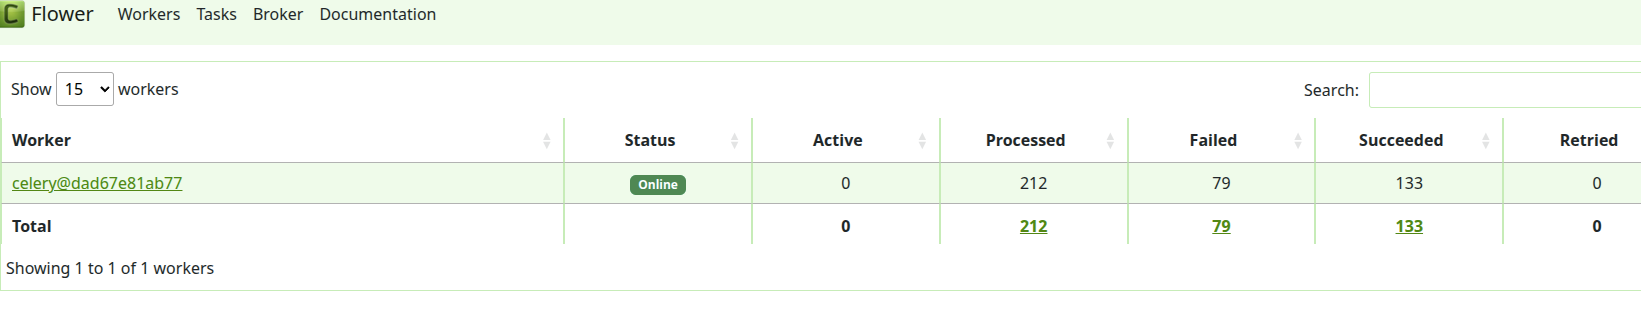
\includegraphics[width=0.85\textwidth]{ch4/assets/flower_ui_feedback.png}
    \caption{Flower Monitoring Dashboard showing Successful and Failed Training Tasks}
    \label{fig:flower_ui_feedback}
\end{figure}

As shown in Figure~\ref{fig:flower_ui_feedback}, a total of 212 training tasks were executed, of which 133 completed successfully and 79 failed. 
The failed tasks were due to unexpected formatting, inconsistencies in the taxonomy labels, such as trailing whitespaces, casing differences, or unexpected variants not previously seen by the model during training or in the training data set.

It is also important to note that although 519 tickets were processed, only 212 training tasks were recorded. 
This discrepancy is due to the fact that the Flower monitoring dashboard is only displaying tasks executed in the last 4 days of the test period, which corresponds to the deployment of the latest stable release of the system. 
As such, earlier training attempts are not visible in the current view but were processed during prior system iterations.

\subsubsection{Evaluation of Overfitting and Underfitting Patterns}

A key objective during evaluation was to determine whether the model exhibited signs of overfitting or underfitting, especially when exposed to live, real-world data that diverged from the training distribution.

All these results are detailed in Appendix~\ref{AppendixB}, Tables~\ref{tab:live_priority_metrics} and~\ref{tab:live_taxonomy_metrics}.

In the local test environment, both priority and taxonomy models achieved high levels of performance. 
Version 11 reached 90\% accuracy on both tasks, with balanced precision and recall across most classes, even those with lower support. 
This indicated strong generalization within the boundaries of a dataset.

However, the transition to the live environment exposed several weaknesses that suggest underfitting in certain areas and potential overfitting in others. 
During live testing, the overall accuracy dropped to 47\% for priority and 41\% for taxonomy, with a pronounced decline in performance on underrepresented classes.

For priority classification, P1 tickets showed the weakest performance, with a recall of only 13\%. 
This contrasts sharply with its recall of 91\% in offline testing. 
Given that P1 tickets were rare both in the training set and in production, this drop indicates underfitting: the model was not sufficiently exposed to the characteristics of these alerts to generalize effectively.

In taxonomy classification, classes such as “Vulnerable” and “Information Gathering” received zero recall, suggesting the model could not recognize or generalize from the limited examples it had seen during training. 
This outcome suggests the oversampling techniques applied during local training were not sufficient to address the imbalance when faced with more diverse, noisy live data. 
These classes appear to have been memorized during training but failed to be correctly identified when presented in a different context, behavior typically associated with overfitting.

Conversely, taxonomy classes like “Malicious Code” and “Fraud”, which had high representation in the training set and continued presence in the live data, maintained relatively stronger performance. 
This supports the idea that the model retained generalization capabilities for dominant classes but struggled to scale that performance to edge cases.

Overall, these results point to a mixed behavior: overfitting in low-support classes that failed to generalize outside of the training data distribution, and underfitting in critical classes like P1, which did not receive enough exposure during training to support accurate predictions in production. 
This highlights the need for more robust class balancing strategies, better augmentation of rare categories, and longer RL adaptation windows to mitigate the limitations of the static RF model and improve long-term generalization.

\subsection{Final Analysis}

The deployment and evaluation of the hybrid RF+RL model revealed both encouraging strengths and critical areas for improvement.

On the positive side, the system demonstrated the feasibility of deploying a containerized, real-time classification pipeline integrated with existing SOC workflows. 
The initial Random Forest model achieved high accuracy and recall in controlled environments, and the end-to-end feedback loop with IBM QRadar SOAR functioned as intended, enabling continuous learning via analyst input.

However, the transition to live data exposed several limitations. 
The most notable issues were a sharp drop in performance on minority classes, inconsistent feedback labeling, and insufficient time for the RL model to adapt. 
These limitations affected both precision and generalization, especially for rare or noisy categories.

To address these challenges, several strategies are proposed:
\begin{itemize}
    \item Improve class balancing through more sophisticated data augmentation or synthetic generation of minority class samples.
    \item Normalize and sanitize feedback labels before training to reduce inconsistencies.
    \item Extend the live evaluation period to allow the RL model to accumulate sufficient training data and stabilize learning.
    \item Monitor per-class performance continuously to trigger targeted retraining when specific categories degrade.
\end{itemize}

The system's architecture and workflow proved operationally viable, but model generalization in production remains an open challenge requiring further refinement and sustained adaptation.


